% Demo a DOS columnas: basta con anadir la opcion de clase estandar de
% LaTeX "twocolumn". \maketitle detecta el modo y saca el bloque de titulo
% a ancho completo por encima de las dos columnas, igual que hace
% article.cls por defecto. Para floats a ancho completo (dos columnas) en
% documentos mas largos, usar los entornos estandar "figure*"/"table*" --
% ver el aviso en uc3mtight.sty sobre por que la figura de esta demo usa
% en cambio un "figure" normal (ancho de una columna).
%
% Con mas texto que main.tex (una columna), a proposito: el sentido de dos
% columnas es aprovechar mas contenido del que cabria en una columna; con
% el mismo texto corto de main.tex, la segunda columna quedaria vacia sin
% que eso sea un fallo de la plantilla, solo falta de texto.
\documentclass[10pt,twocolumn]{article}

\usepackage[spanish,es-noquoting]{babel}
\usepackage{uc3mtight}

\title{Resumen: caché de resultados en la capa de consultas}
\subject{Bases de Datos}
\group{Grupo 84}
\author{Raúl Aguilar Arroyo \and Ana Pérez Ruiz}
\date{Curso 2026/2027}

\begin{document}
\maketitle

\section{Motivación}

El coste de recalcular consultas repetidas sobre el mismo conjunto de datos
motiva introducir una capa de caché entre la aplicación y el motor de base
de datos, reduciendo la latencia percibida sin modificar el esquema
subyacente. En sistemas con una proporción alta de lecturas frente a
escrituras, una fracción significativa de las consultas repite exactamente
los mismos parámetros en ventanas de tiempo cortas, lo que hace que el
coste de mantener una caché quede sobradamente compensado por el ahorro en
tiempo de cómputo del motor relacional.

\subsection{Planteamiento}

Se evalúa una caché LRU en memoria situada delante del motor relacional,
invalidada de forma explícita en cada escritura sobre las tablas afectadas.
La clave de caché se construye a partir de la consulta parametrizada y sus
argumentos, de modo que dos invocaciones equivalentes con los mismos
parámetros comparten entrada aunque provengan de peticiones HTTP distintas.

\subsubsection{Alcance} Este resumen cubre únicamente el caso de consultas
de solo lectura sobre una única tabla; los joins multi-tabla quedan fuera
del análisis presentado aquí.

\section{Trabajo relacionado}

Las estrategias de invalidación de caché suelen dividirse en tres familias:
por tiempo de vida fijo (TTL), por notificación explícita del origen de
datos, e híbridas. El enfoque por TTL es el más sencillo de implementar
pero introduce una ventana de inconsistencia entre la escritura y la
expiración de la entrada; el enfoque por notificación, el usado aquí, evita
esa ventana a costa de acoplar la caché al camino de escritura.

Ventajas e inconvenientes de cada familia:
\begin{itemize}
  \item \textbf{TTL fijo}: implementación trivial, pero puede servir datos
  obsoletos durante la ventana de expiración.
  \item \textbf{Notificación explícita}: consistencia inmediata, pero
  requiere instrumentar todos los caminos de escritura.
  \item \textbf{Híbrido}: combina un TTL largo como red de seguridad con
  notificación explícita como mecanismo principal.
\end{itemize}

\section{Resultados}

La \autoref{tab:resultados} resume la reducción de latencia observada para
distintos tamaños de caché.

\begin{table}[h]
  \centering
  \caption{Latencia media según tamaño de caché.}
  \label{tab:resultados}
  \begin{tabular}{@{}lrr@{}}
    \toprule
    Tamaño caché & Latencia (ms) & Aciertos (\%) \\
    \midrule
    Sin caché & 42 & --- \\
    128 entradas & 19 & 61 \\
    512 entradas & 8 & 89 \\
    \bottomrule
  \end{tabular}
\end{table}

Ventajas observadas:
\begin{itemize}
  \item Reducción de latencia media superior al 80\,\% con 512 entradas.
  \item Sin cambios en el esquema ni en las consultas de la aplicación.
\end{itemize}

La \autoref{fig:latencia} ilustra la tendencia.

\begin{figure}[h]
  \centering
  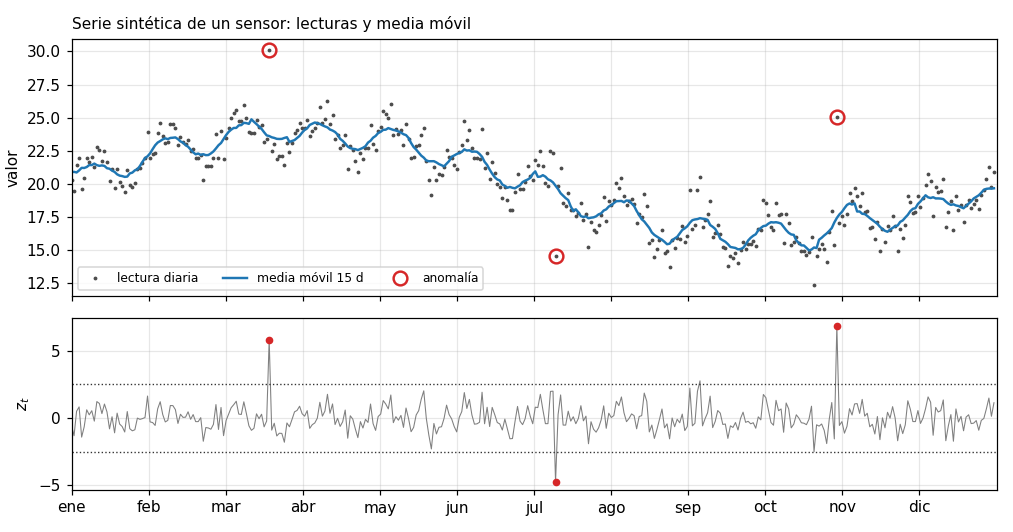
\includegraphics[width=\linewidth]{figs/demo-figura}
  \caption{Latencia media en función del tamaño de la caché.}
  \label{fig:latencia}
\end{figure}

\section{Conclusión}

Una caché LRU sencilla, invalidada por escritura, ofrece una reducción de
latencia sustancial con una complejidad de implementación baja, siempre que
las consultas se limiten a lecturas de una sola tabla. Extender el enfoque
a joins multi-tabla exigiría invalidar por cada tabla involucrada en la
consulta, lo que queda propuesto como trabajo futuro.

\end{document}
